%%%%%%%%%%%%%%%%%%%%%%%%%%%%%%%%%%%%%%%%%%%%%%%%%%%%%%%%%%%%%%%%%%%%%%
%     File: ExtendedAbstract_imple.tex                               %
%     Tex Master: ExtendedAbstract.tex                               %
%                                                                    %
%     Author: Andre Calado Marta                                     %
%     Last modified : 27 Dez 2011                                    %
%%%%%%%%%%%%%%%%%%%%%%%%%%%%%%%%%%%%%%%%%%%%%%%%%%%%%%%%%%%%%%%%%%%%%%
% A Calculation section represents a practical development
% from a theoretical basis.
%%%%%%%%%%%%%%%%%%%%%%%%%%%%%%%%%%%%%%%%%%%%%%%%%%%%%%%%%%%%%%%%%%%%%%

\section{Results}
\label{sec:imple}
\vspace{0.5cm}
\subsection{Stabilization}
Determinant Quantum Monte Carlo suffers from low temperature and large size numerical instabilities.
These arise because the information about the quantum states we seek is encoded in the differences between matrix elements of largely different magnitude contained in the elements of the $\bm B$-matrices of Eq.(\ref{eq:Z_quadratic}).
It is outside of the scope of this document to describe the stabilization procedure (it is done in the thesis).
In short, we find the energy scales that gives us the relevant information we seek via a $\bm Q \bm R$ decomposition with partial pivoting (following \cite{bai_stable_2011}), and then we cut off the irrelevant scales that destabilize the matrix products we need to compute, using a matrix $\bm D'$ (the notation becomes clear in the thesis).
\begin{figure}[H]
  \centering
  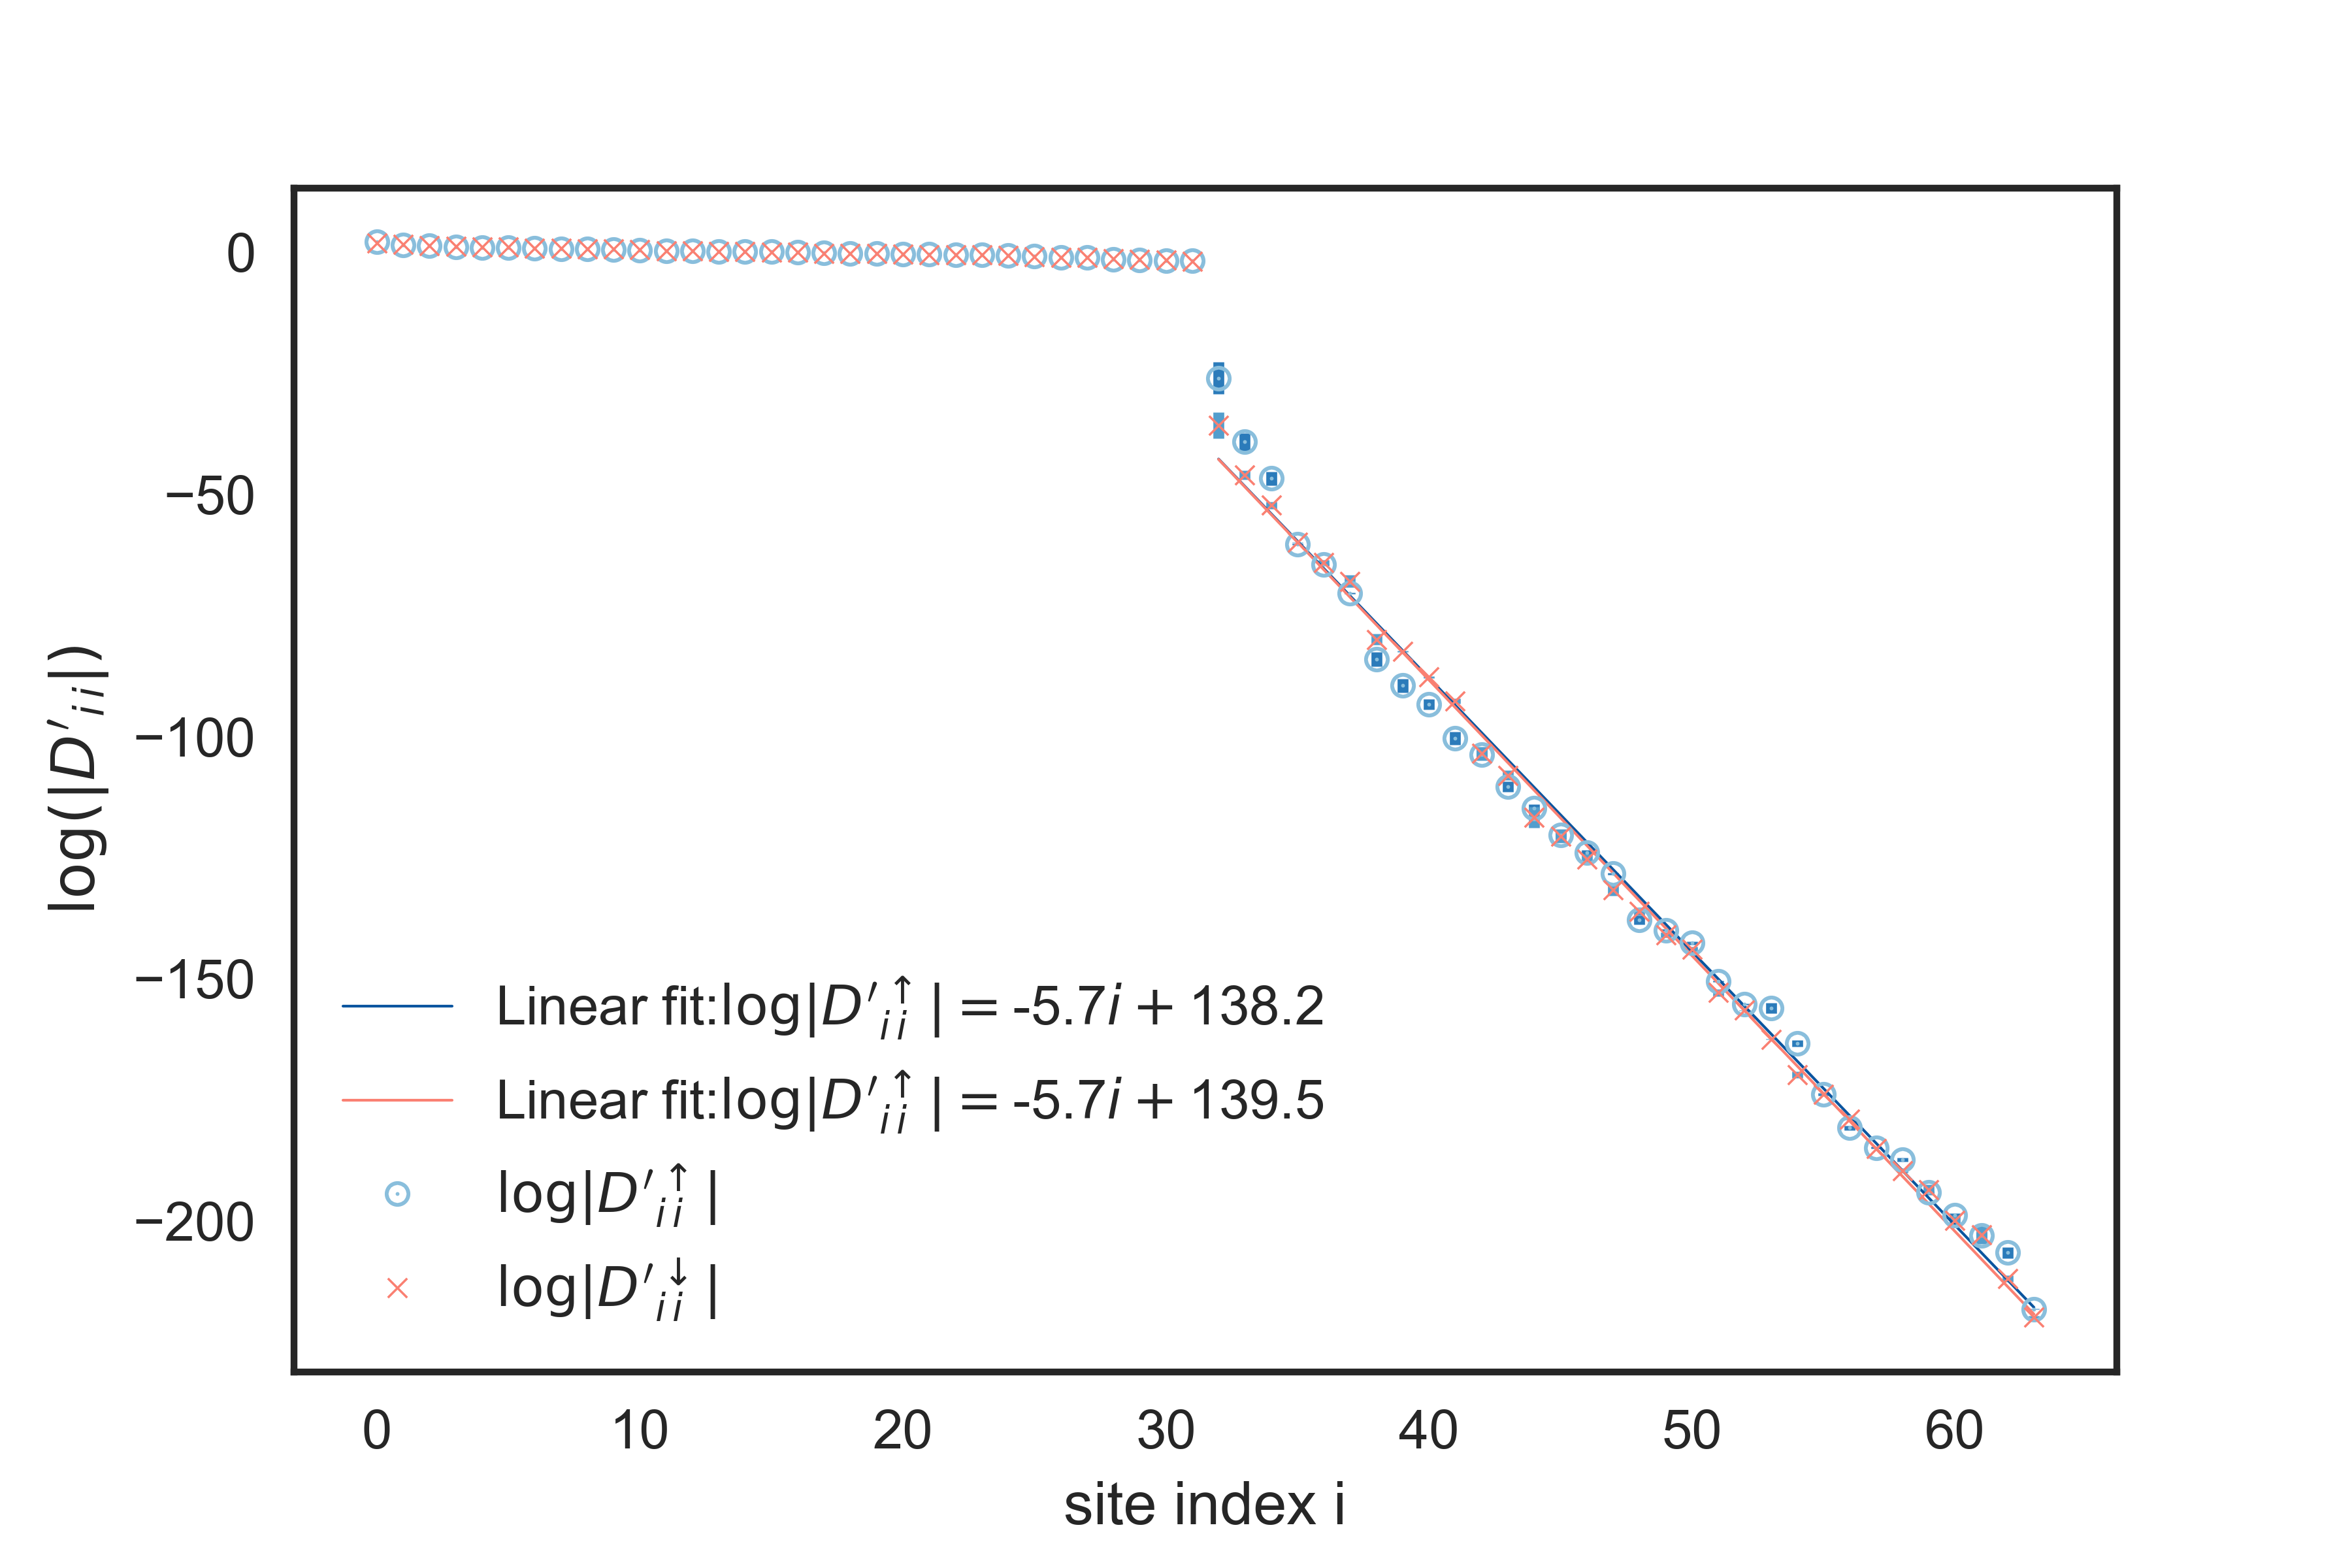
\includegraphics[width =7.5cm]{images/OrdersOfMagnitude_N=64sites.png}
  \caption{The matrix $\bm D'$ (standard notation used in the thesis) displays the scales spanned by the stably multiplied $\bm B$-matrices (in this case for $\beta = 20t$, $U = 8t$, on a 64-site 1D chain with periodic boundary conditions).}
  \label{fig:numerical_scales}
\end{figure}
\subsection{Benchmarks}
Our comparison with the auxiliary field QMC results of \texttt{QUEST} for a 64-site 1D chain with periodic boundary conditions with $U = 4 t$, and $\beta = 25 t$, shows remarkable agreement, namely in the magnetic structure factor.
\begin{figure}[H]
  \centering
  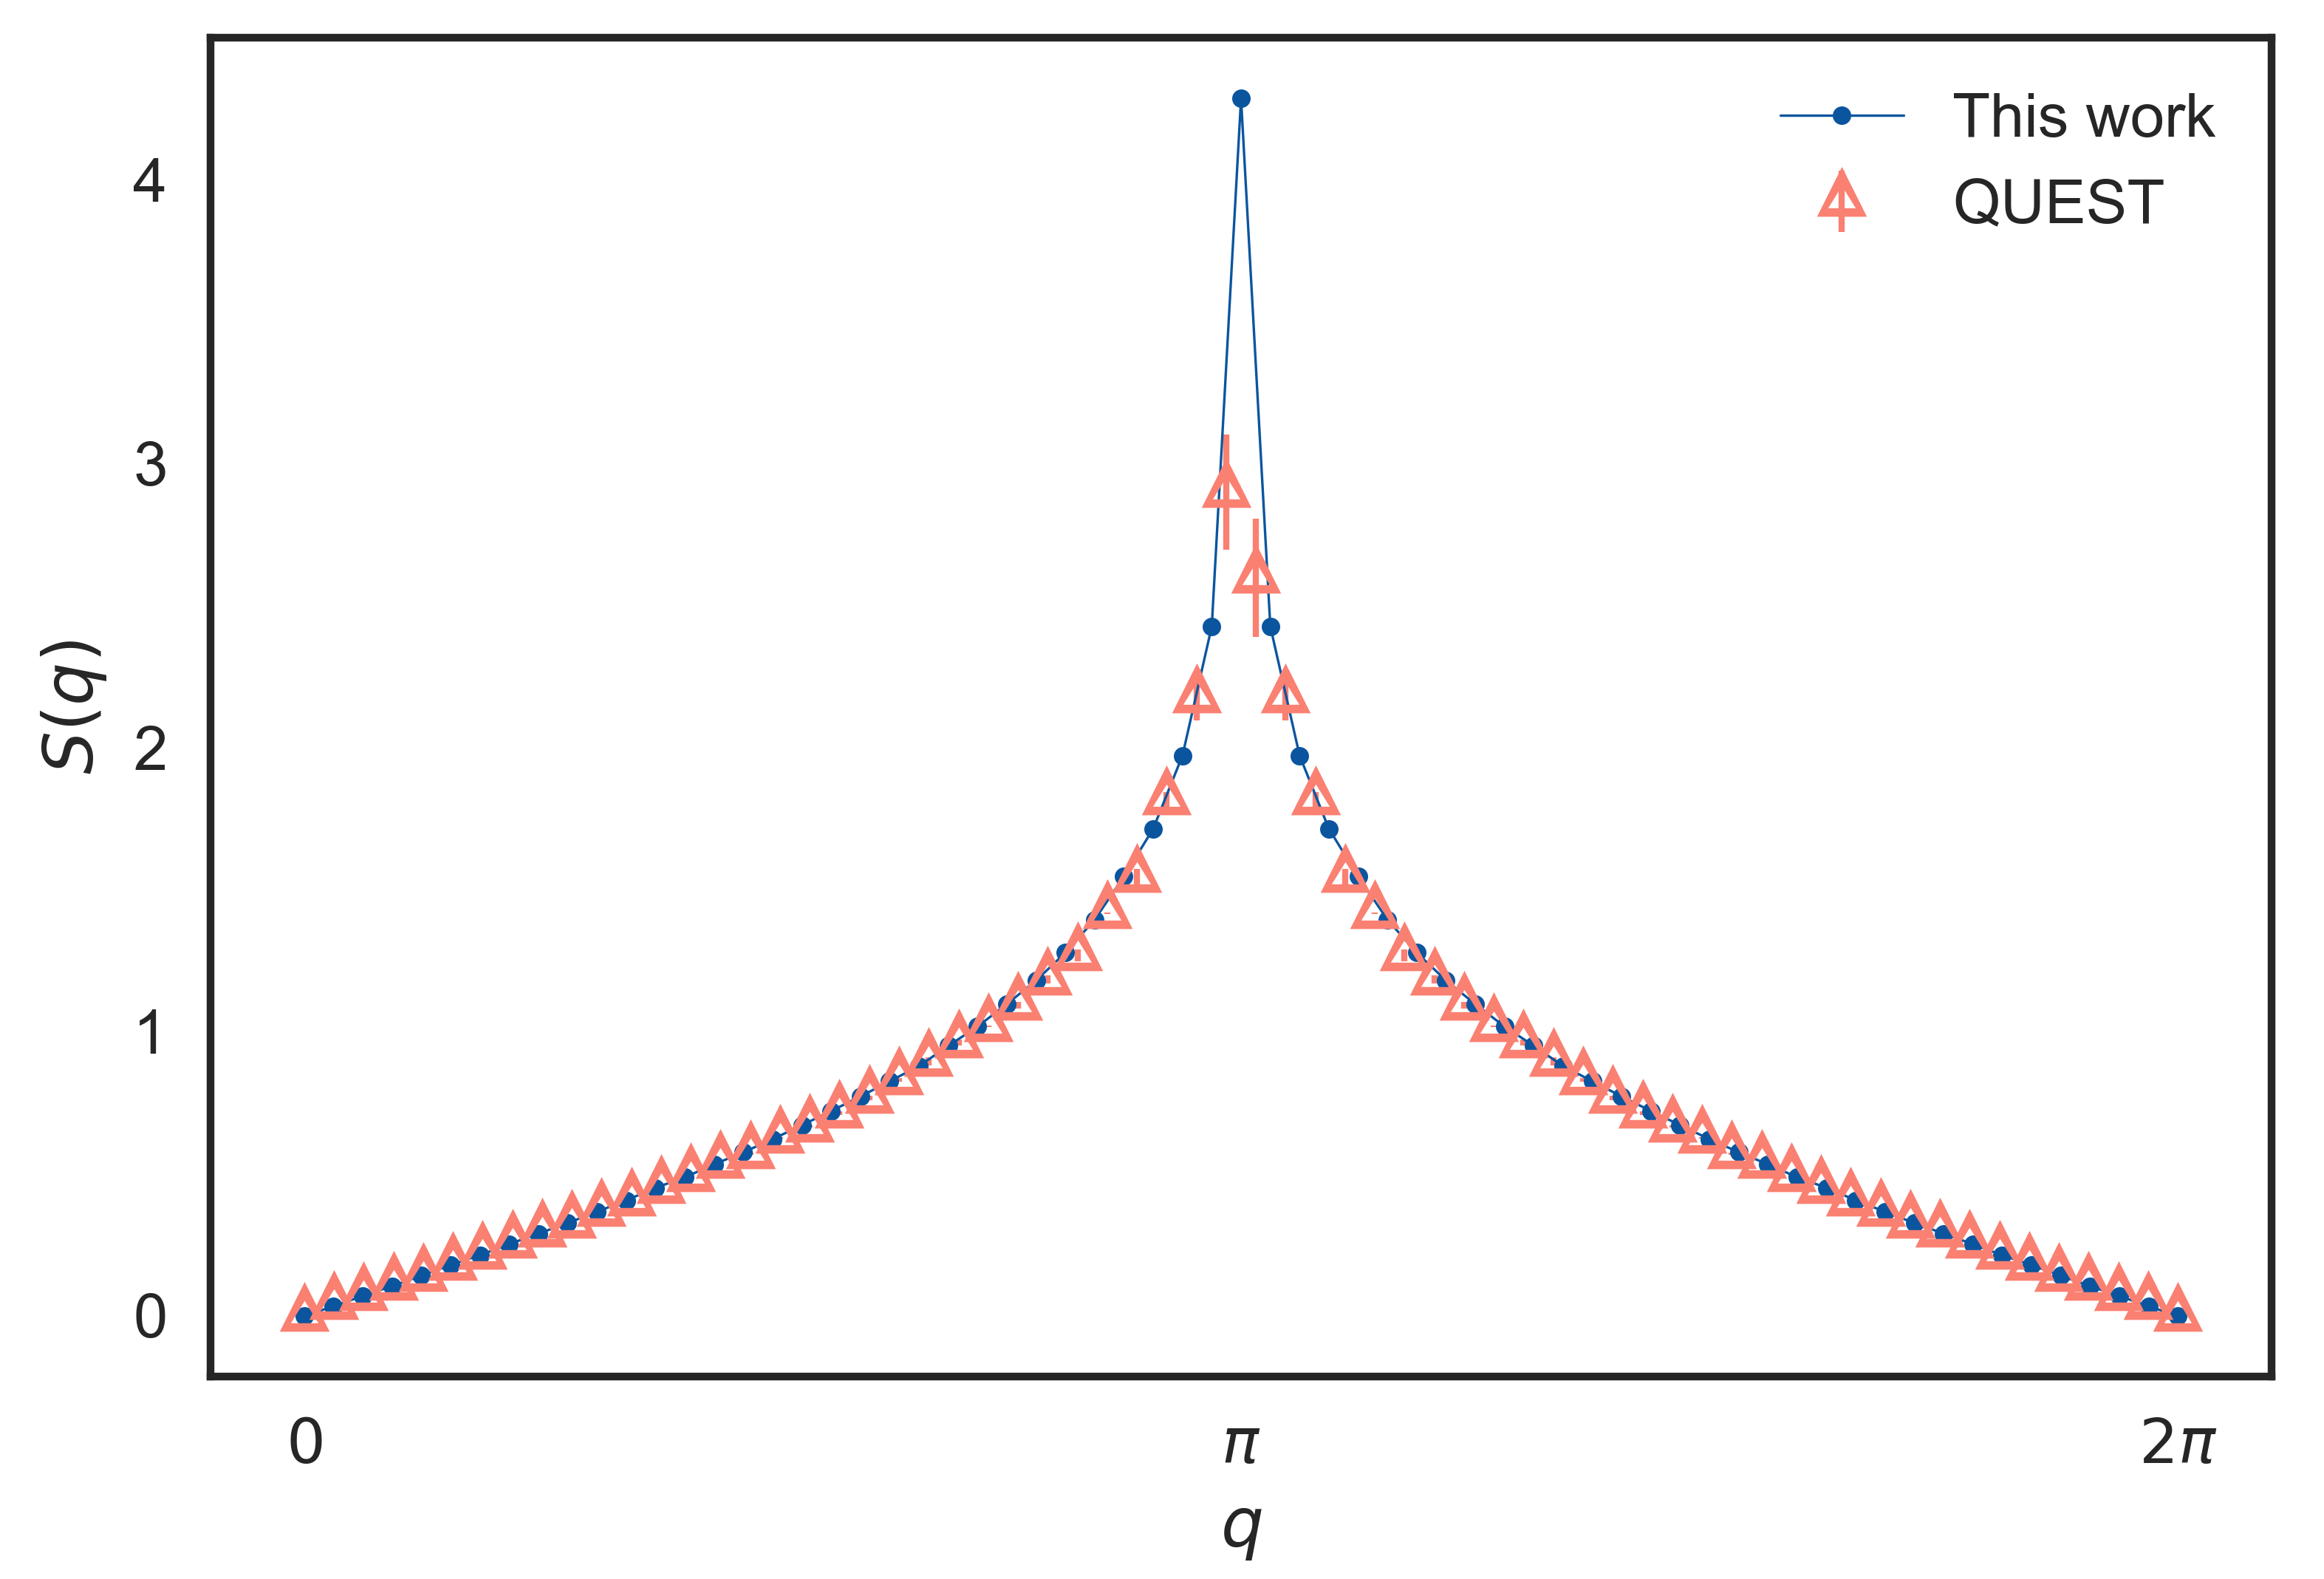
\includegraphics[width=7.5cm]{images/s_compare.png}
  \caption{Comparison between our measurement magnetic structure factor and the result obtained when we ran  \texttt{QUEST}}
  \label{figdetVSquest}
\end{figure}
Another benchmark is the result that we obtain for the magnetic ordering in a strained graphene nanoribbon, reproducing the results of a recent paper \cite{yang_strain-tuning_2017}.
The prediction of our mean field calculation for a strained graphene nanoribbon (with hoppings reduced along its longitudinal $x$ direction $t \mapsto t - \Delta, \Delta = 0.3t$) is that the spins along the rows of the ribbon have uniform correlation.
In fact, we can see that mean field overestimates long range ordering, and they follow instead the symmetric profile of Fig.(\ref{fig:corrProf}), a behavior typical of this type of graphene-based system \cite{feldner_dynamical_2011, raczkowski_interplay_2017}.
This result expands on the study carried out in \cite{yang_strain-tuning_2017}.
\begin{figure}[H]
  \centering
  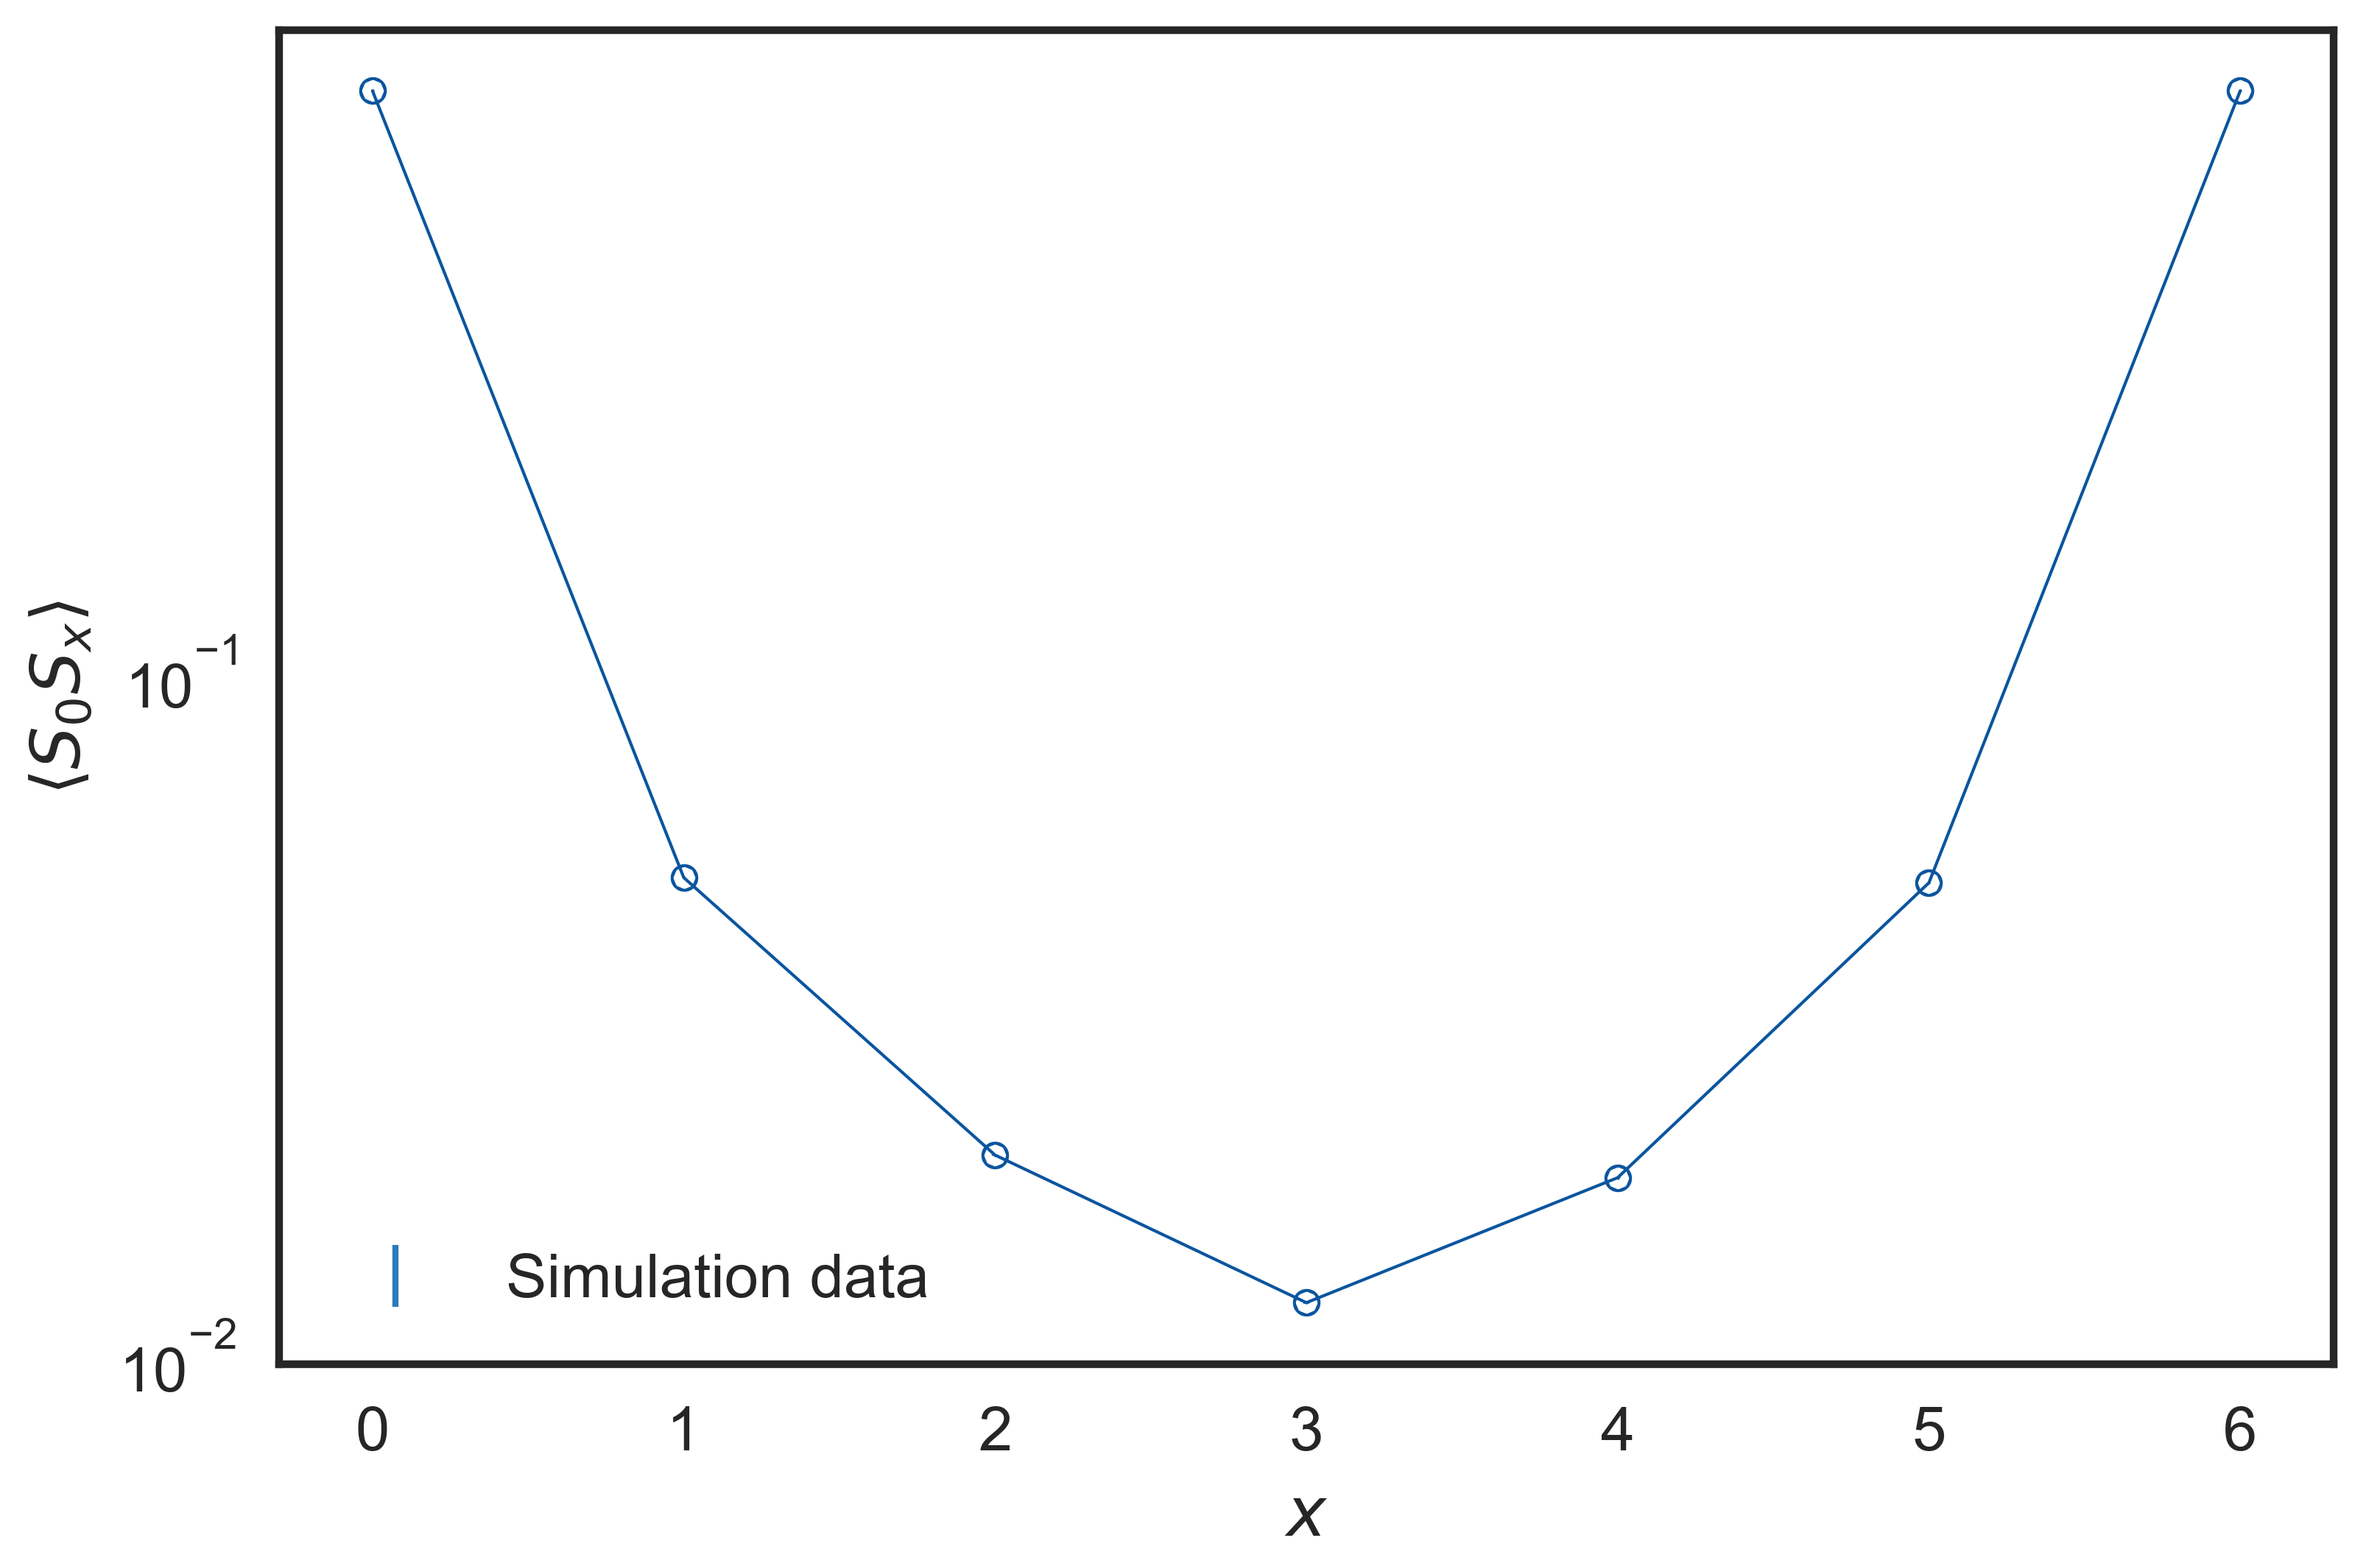
\includegraphics[width = 7.5cm]{images/LongitudinalProfile.png}
  \caption{Profile of the spin-spin correlations along the edge for a $ 6 \times 6$ strained graphene nanoribbon at $\beta = 16$, $U = 3t$, $\Delta = 0.3$.}
  \label{fig:corrProf}
\end{figure}
By computing the susceptibility on the edge (restricting the sum in Eq.(\ref{eq:chi}) to sites on the edge) for one of the sublattices, we are to find the critical temperature for the transition to the ordered state for $U = 3 t$, $T_c = ( 0.017 \pm 0.003 ) t$.
This is done by fitting the results for the susceptibility obtained for our simulates run at different temperatures to the Curie Law $\chi \propto ( T - T_c )^{-1}$ (see Fig.(\ref{fig:chiFit}).
Repeating the procedure for varying temperature, and on-site interaction, we would be able to draw a complete phase diagram.
\begin{figure}[H]
  \centering
  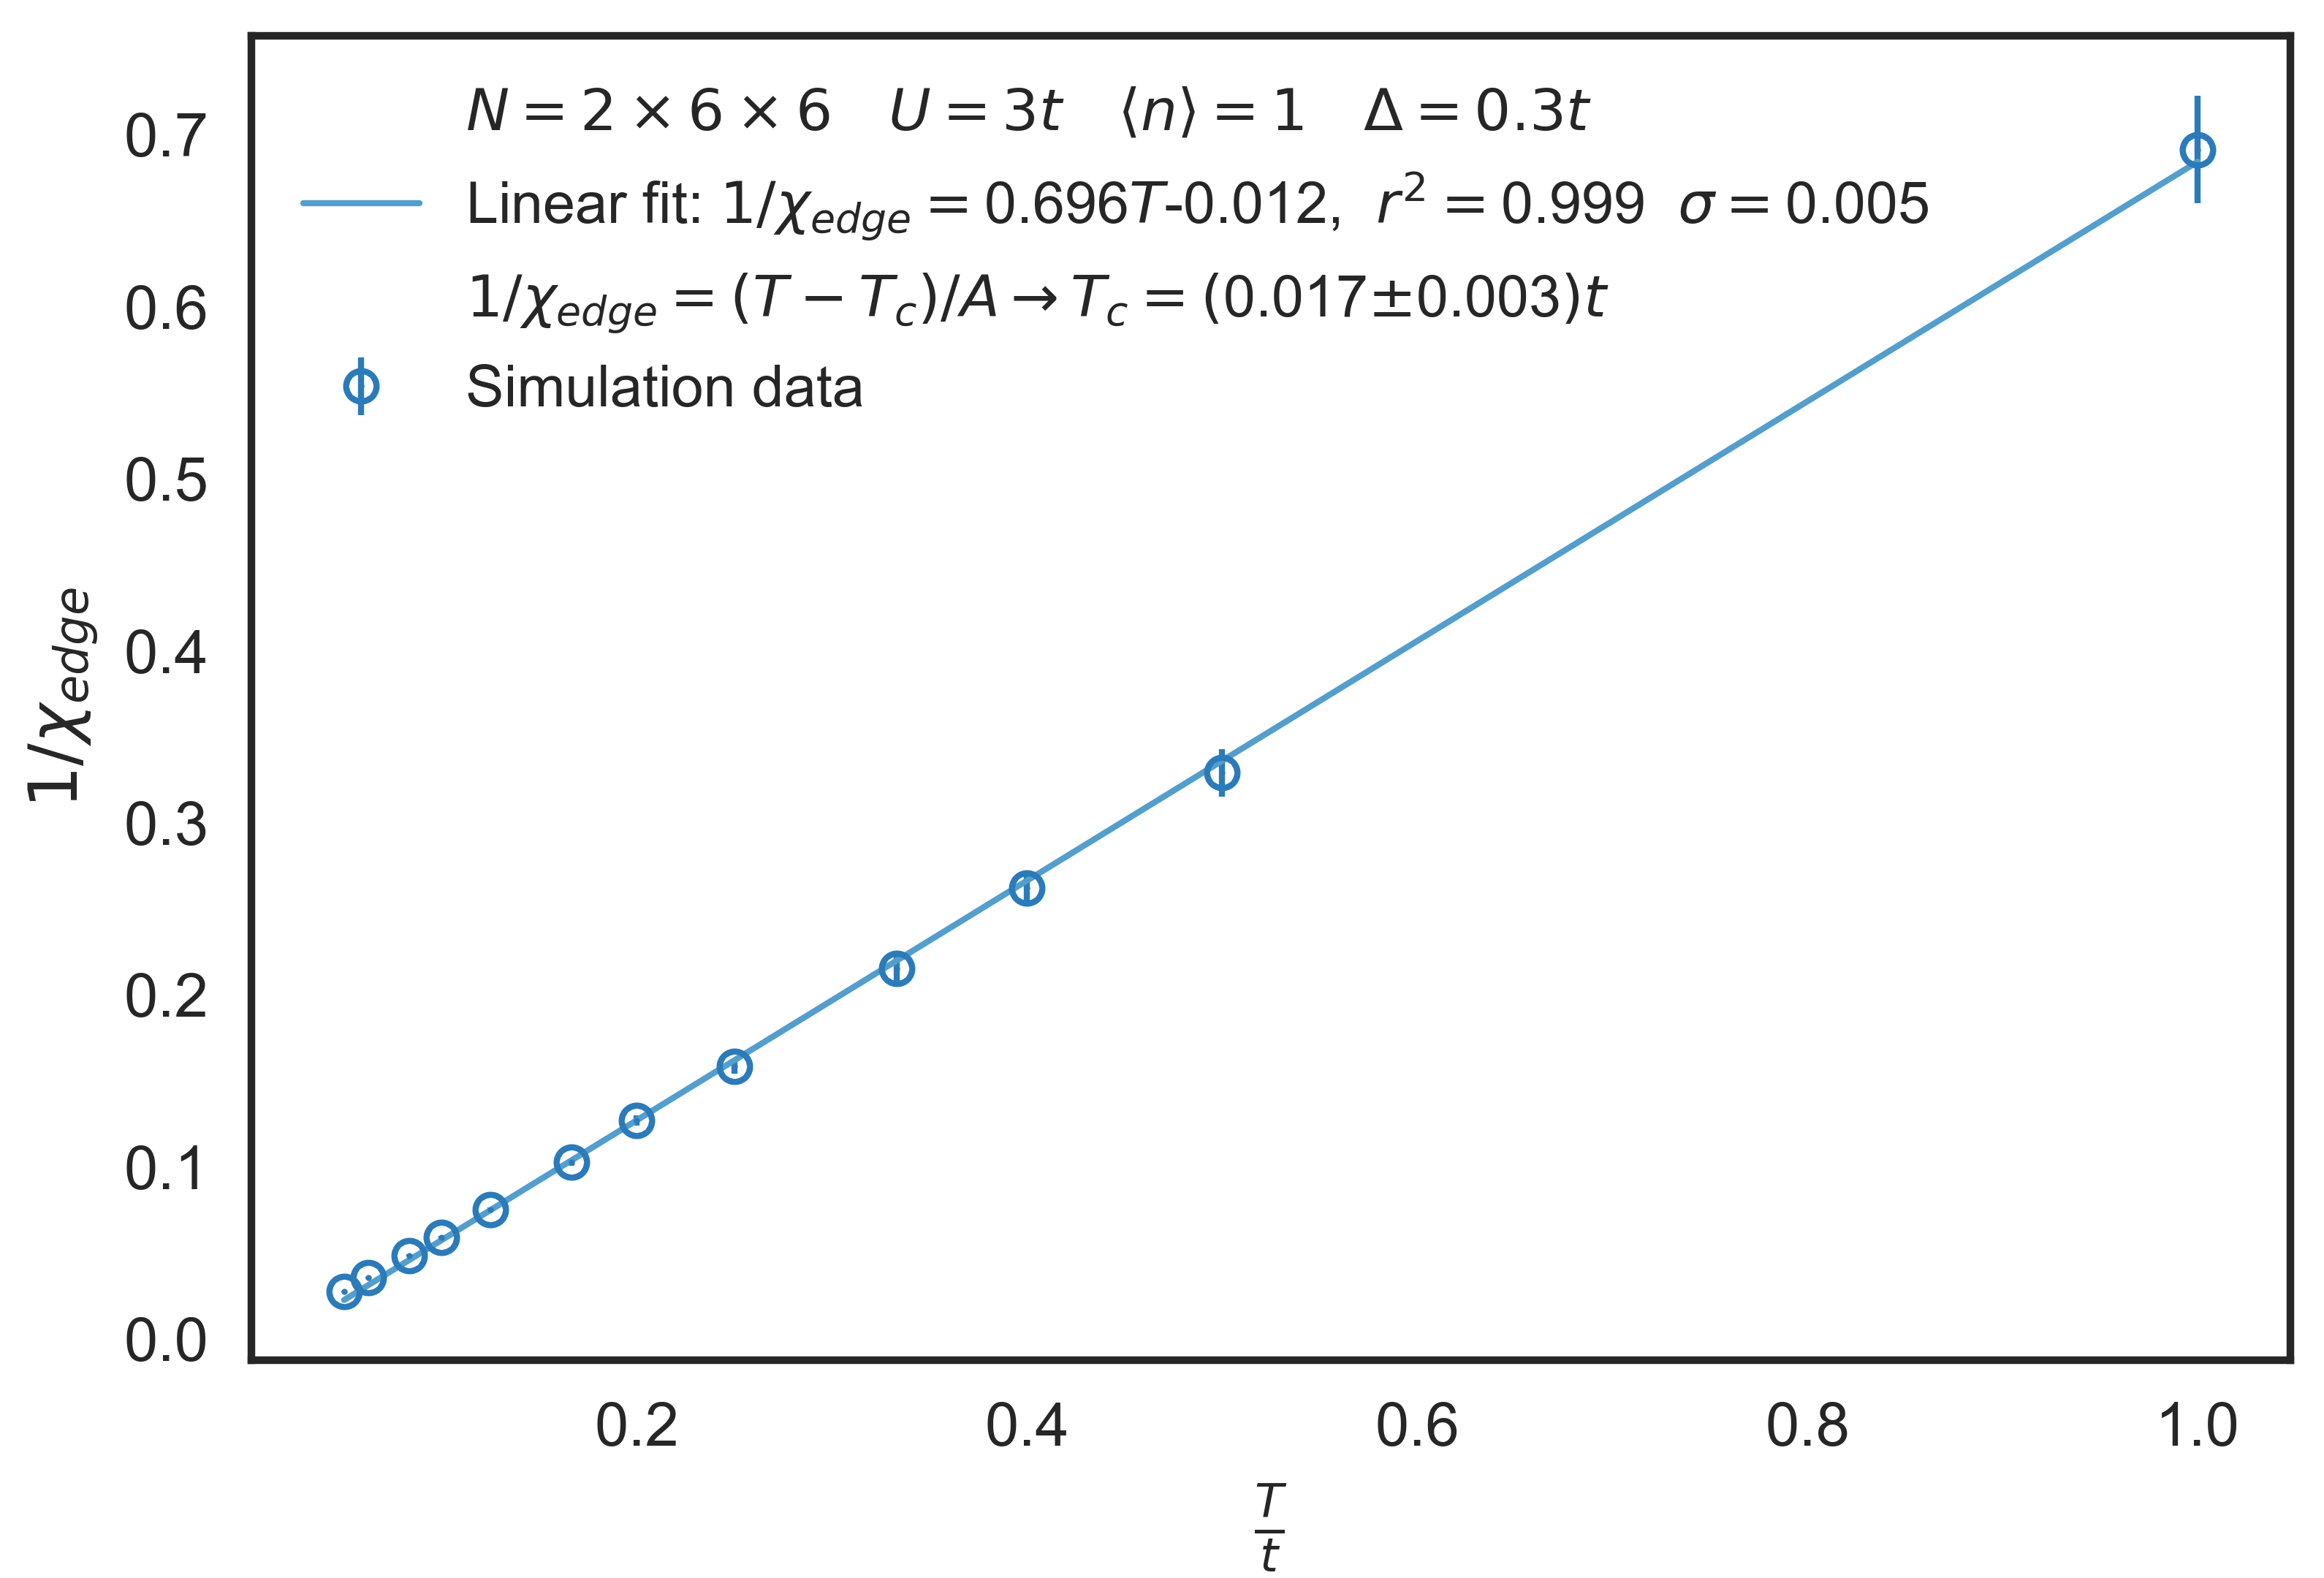
\includegraphics[width=7.5cm]{images/fityang2017.png}
  \caption{Fit of $\chi_{\text{edge}} to Curie's Law$.}
  \label{fig:chiFit}
\end{figure}


%%%%%%%%%%%%%%%%%%%%%%%%%%%%%%%%%%%%%%%%%%%%%%%%%%%%%%%%%%%%%%%%%%%%%%



